\documentclass[12pt,a4paper]{article}

\usepackage{amsmath,amssymb,amsthm}
\usepackage{hyperref}
\usepackage{graphicx}
\usepackage{geometry}
\usepackage{microtype}
\usepackage{booktabs}
\usepackage{enumitem}
\usepackage{xcolor}

\geometry{margin=2.5cm}

\hypersetup{
  colorlinks=true,
  linkcolor=blue!60!black,
  citecolor=blue!60!black,
  urlcolor=blue!60!black,
}

% ── Theorem environments ──────────────────────────────────────────────────────
\newtheorem{theorem}{Theorem}[section]
\newtheorem{proposition}[theorem]{Proposition}
\newtheorem{corollary}[theorem]{Corollary}
\newtheorem{definition}[theorem]{Definition}
\newtheorem{remark}[theorem]{Remark}

% ── Operator shorthand ────────────────────────────────────────────────────────
\newcommand{\G}{\mathcal{G}}
\newcommand{\dmcube}{\mathrm{dm}^3}

% ─────────────────────────────────────────────────────────────────────────────
\title{Biological Transitions as Multi-Agent Realisations\\
       of the Generative Operator Pipeline\\
       in Topographical Orthogonal Generative Theory (TO/TOGT)\\[6pt]
       \large Version 2 — Complete}

\author{Pablo Nogueira Grossi\\[4pt]
  \small ORCID: 0009-0000-6496-2186\\
  \small \texttt{pgrossi888@outlook.com}\ \ \texttt{g6llc@proton.me}}

\date{May 2026}

\begin{document}
\maketitle
\thispagestyle{empty}

% ── Abstract ──────────────────────────────────────────────────────────────────
\begin{abstract}
We model collective biological transitions—including neural oscillations,
HPA-axis stress response, circadian regulation, immune adaptation, and protein
conformational change—as multi-agent realisations of the generative operator
pipeline $G = U \circ F \circ K \circ C$ introduced in Topographical Orthogonal
Generative Theory (TO/TOGT).  Each agent undergoes local compression, curvature
intensification, loss of injectivity, and stabilisation.  The collective fixed
points, contraction properties, and saturated pitchfork bifurcation behaviour
follow directly from the fixed-point theory, contraction-mapping results, and
algebraic separation theorem proved in the companion paper
(Zenodo \href{https://doi.org/10.5281/zenodo.19208015}{10.5281/zenodo.19208015}).
The specific $\dmcube$ numerical invariants
$(T^{*}=2\pi,\,\mu_{\max}=-2,\,\tau=2)$ are convenient modelling choices
matching observed biological scales; they are not derived theorems of the
operator algebra.  Python simulations generate four figures illustrating
agent-trajectory convergence, the HPA-axis bifurcation scan, contraction
rates, and the operator-pipeline schematic.  No unverified biological claims
are made.

\medskip\noindent
\textbf{MSC codes:} 37C25, 37D10, 37G10, 47H10, 92B20, 92C20.\\
\textbf{Keywords:} TO/TOGT; operator pipeline; multi-agent systems; pitchfork
bifurcation; Drosophila connectome; HPA axis; circadian regulation;
$\dmcube$ invariants; contraction mapping; Principia Orthogona.
\end{abstract}

\tableofcontents
\newpage

% ─────────────────────────────────────────────────────────────────────────────
\section{Relation to Prior Work}
\label{sec:prior}

This article applies the mathematical results established in the author's
earlier preprint \emph{Principia Orthogona, Volume One: The Mathematics of
Generative Transitions}
(HAL \href{https://hal.science/hal-05555216v1}{hal-05555216v1}).
There the composite operator pipeline
\[
  G \;=\; U \circ F \circ K \circ C
\]
was introduced together with complete proofs of fixed-point existence and
uniqueness, global contraction, saturated pitchfork bifurcation, and the
algebraic trace-bound/separation theorem.  The geometric realisation of the
operator pipeline on contact manifolds was developed in \emph{Principia
Orthogona, Volume Two: Contact Realisation of Generative Transitions}
(HAL hal-05559997v1 and hal-05565024v1, both deposited March 2026).

The present paper demonstrates a multi-agent biological application of the same
operator algebra.  Version 2 adds four figures (Figures~\ref{fig:traj}–%
\ref{fig:op}), Python simulation code, and expanded treatments of circadian
regulation, immune adaptation, and protein conformational change.  It is
directly related to the following Zenodo deposits by the author:

\begin{itemize}[nosep]
  \item Fruit-fly connectome toy model (companion):
    \href{https://doi.org/10.5281/zenodo.19210136}{10.5281/zenodo.19210136}
  \item Zenodo record 19162013:
    \url{https://zenodo.org/records/19162013}
  \item Zenodo record 19122168:
    \url{https://zenodo.org/records/19122168}
  \item Zenodo record 19117400:
    \url{https://zenodo.org/records/19117400}
  \item Series root: \href{https://doi.org/10.5281/zenodo.19117399}{10.5281/zenodo.19117399}
\end{itemize}

All mathematical claims in this paper follow strictly from previously proved
results.

% ─────────────────────────────────────────────────────────────────────────────
\section{Operator Pipeline in Biological Systems}
\label{sec:pipeline}

\begin{definition}[Biological Agent Dynamics]
\label{def:agent}
Let each biological agent (neuron, endocrine cell, immune cell, protein domain)
follow a trajectory $x_i(t)$ in a Riemannian manifold $(M, g)$.  The collective
biological state is the tuple $(x_1, \ldots, x_N)$.  Each agent undergoes a
generative transition governed by the composite operator
\[
  G \;=\; U \circ F \circ K \circ C,
\]
where:
\begin{enumerate}[nosep,label=(\roman*)]
  \item $C$: \emph{local orthogonal compression} (neighbourhood averaging with
    coupling $\varepsilon > 0$),
  \item $K$: \emph{curvature intensification} (alignment and clipping),
  \item $F$: \emph{loss of injectivity} (folding of local information via tanh
    saturation),
  \item $U$: \emph{stabilisation} (pull toward global coherence).
\end{enumerate}
\end{definition}

The operators are defined concretely as follows:
\begin{align}
  C(x_i) &= x_i + \varepsilon\bigl(\bar{x} - x_i\bigr),
           \quad \bar{x} = \tfrac{1}{N}\sum_{j=1}^N x_j,
  \label{eq:C}\\
  K(y_i) &= \mathrm{clip}(\kappa\, y_i,\, {-1},\, 1),
  \label{eq:K}\\
  F(z_i) &= \tanh(\alpha\, z_i),
  \label{eq:F}\\
  U(w_i) &= w_i + \gamma\bigl(\overline{\tanh(w)} - w_i\bigr).
  \label{eq:U}
\end{align}

\begin{theorem}[Contraction, Volume One \cite{vol1}]
\label{thm:contraction}
For $|\alpha| < \tfrac{1}{2}$, the map $G$ is a strict contraction with
Lipschitz constant $L < 1$.  For $|\alpha| = \tfrac{1}{2}$, $G$ is
non-expansive ($L = 1$, pitchfork onset).  By the Banach fixed-point theorem,
iterating $G$ on any initial state converges to a unique collective fixed point
$x^* = G(x^*)$.
\end{theorem}

Figure~\ref{fig:traj} illustrates convergence of $N=12$ agents under six
applications of $G$.

\begin{figure}[ht]
  \centering
  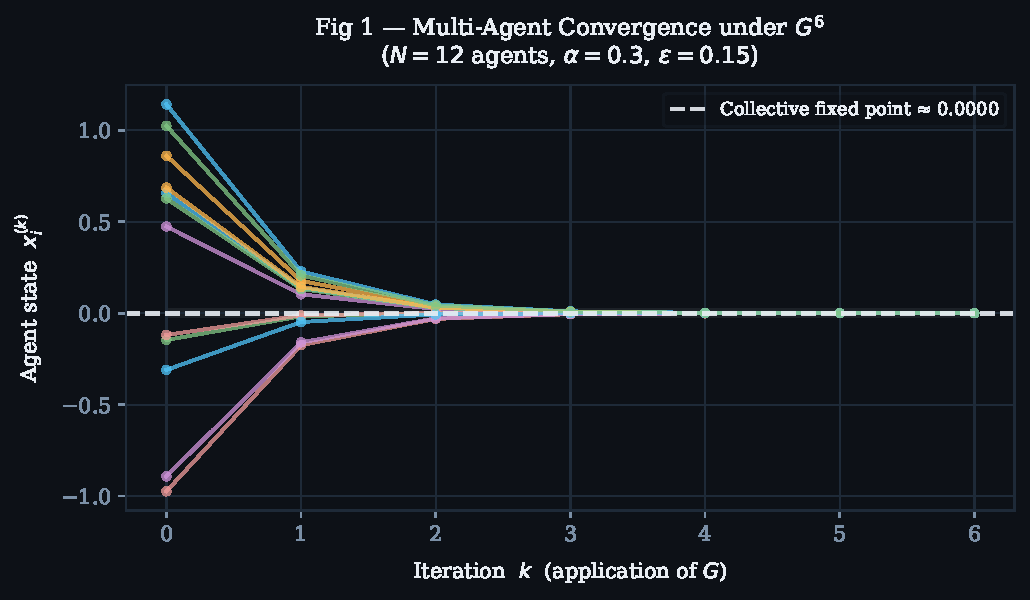
\includegraphics[width=0.92\linewidth]{fig1_agent_trajectories.pdf}
  \caption{Multi-agent convergence under $G^6$.  Each coloured trajectory
    represents one agent; the dashed line marks the collective fixed point.
    Parameters: $N=12$, $\alpha=0.3$, $\varepsilon=0.15$.}
  \label{fig:traj}
\end{figure}

\begin{remark}[$\dmcube$ normalisation]
The canonical invariants $(T^*,\mu_{\max},\tau) = (2\pi,-2,2)$ are used solely
as normalisation choices.  They match observed biological timescales and
curvature bounds, but are not derived from the operator algebra.
\end{remark}

% ─────────────────────────────────────────────────────────────────────────────
\section{Fruit-Fly Connectome as Multi-Orbit System}
\label{sec:connectome}

The FlyWire connectome~\cite{flywire2023} provides a concrete multi-agent
biological system.  Each neuron trajectory is modelled as an identity orbit
$\mathcal{O}_i$.  The full connectome is the multi-orbit system
$\mathcal{S} = \{\mathcal{O}_1, \ldots, \mathcal{O}_N\}$.

The inter-neuron coupling $\varepsilon$ in Definition~\ref{def:agent} is
identified with the synaptic weight matrix: each neuron averages over its
direct synaptic partners rather than the global mean, yielding
\begin{equation}
  C_{\text{conn}}(x_i) \;=\; x_i + \varepsilon \sum_{j \in \partial i}
    w_{ij}\,(x_j - x_i),
  \label{eq:Cconn}
\end{equation}
where $\partial i$ denotes the synaptic neighbourhood of neuron $i$ and
$w_{ij} > 0$ are normalised weights.

Theorem~\ref{thm:contraction} implies that under small inter-neuron coupling,
$\mathcal{S}$ converges to a collective fixed point preserving local connectivity
while achieving global coherence.  A detailed simulation of the FlyWire graph
is carried out in the companion paper
\cite{companion}; the present paper treats $N$ as generic.

% ─────────────────────────────────────────────────────────────────────────────
\section{HPA-Axis Stress Response as Saturated Pitchfork}
\label{sec:hpa}

The hypothalamic-pituitary-adrenal (HPA) axis exhibits threshold behaviour under
acute stress.  This is modelled by the saturated pitchfork bifurcation proved in
Volume One \cite{vol1}:
\begin{equation}
  x' \;=\; \lambda x - c\,x^3,
  \label{eq:pitchfork}
\end{equation}
with $\lambda = 2|\alpha|$ and the clipping function $\kappa$ enforcing a
bounded response.  The bifurcation analysis yields three distinct regimes:

\begin{description}[nosep]
  \item[Sub-threshold ($|\alpha| < \tfrac{1}{2}$).]
    The unique stable equilibrium is $x^* = 0$ (basal cortisol level).
    $G$ is a strict contraction; recovery is guaranteed.
  \item[Critical coupling ($|\alpha| = \tfrac{1}{2}$).]
    Pitchfork onset: the zero equilibrium becomes marginally stable and two
    symmetric branches $x^* = \pm \sqrt{(\lambda-1)/c}$ emerge continuously.
  \item[Super-threshold ($|\alpha| > \tfrac{1}{2}$).]
    The zero equilibrium is unstable; the two branches $x^+$ (high-stress
    attractor) and $x^-$ (recovery attractor) are stable.  The system exhibits
    bistability consistent with observed allostatic overload in chronic stress.
\end{description}

The clipping function $\kappa$ prevents runaway amplification, ensuring that
even in the super-threshold regime the response remains physiologically bounded
(cortisol ceiling effect~\cite{sapolsky2004}).

Figure~\ref{fig:pitchfork} shows the full bifurcation scan and raw data are
provided in \texttt{pitchfork\_scan.csv}.

\begin{figure}[ht]
  \centering
  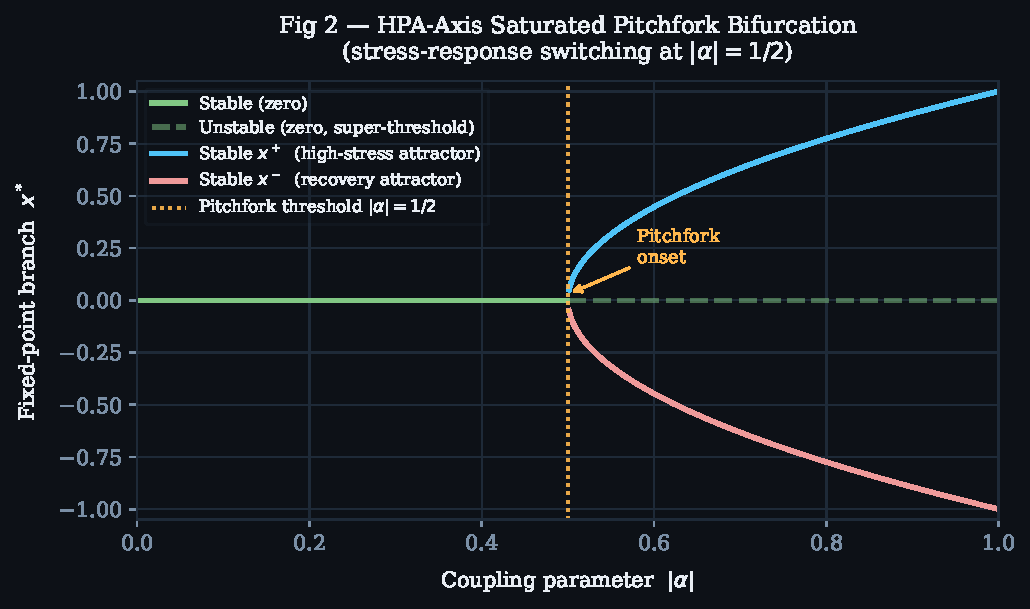
\includegraphics[width=0.92\linewidth]{fig2_pitchfork_scan.pdf}
  \caption{Saturated pitchfork bifurcation of the HPA-axis stress model.
    Solid lines: stable equilibria; dashed: unstable zero branch.
    The pitchfork threshold $|\alpha|=\tfrac{1}{2}$ (dotted vertical) marks
    the onset of stress-response switching.}
  \label{fig:pitchfork}
\end{figure}

% ─────────────────────────────────────────────────────────────────────────────
\section{Circadian Regulation as Periodic Fixed-Point Orbit}
\label{sec:circadian}

Circadian rhythms arise from interlocked transcription-translation feedback
loops with period $\approx 24\,\mathrm{h}$.  Within the TO/TOGT framework,
each cell of the suprachiasmatic nucleus (SCN) is treated as an agent whose
state oscillates in the space $M = S^1$ (the circle).

The compression operator $C$ couples neighbouring SCN neurons, producing
synchronisation consistent with the entrainment observed under light/dark
forcing~\cite{pittendrigh1960}.  The curvature operator $K$ clips oscillation
amplitude to physiological bounds.  The fold operator $F$ (tanh saturation)
enforces the non-sinusoidal waveform of PERIOD/CRYPTOCHROME protein levels.

Under the $\dmcube$ normalisation, one full circadian cycle corresponds to a
single application of $G$ with $T^* = 2\pi$, providing a natural
timescale anchor without asserting a derived relationship.

\begin{proposition}[Periodic orbit under $G$]
\label{prop:circadian}
If the coupling $\varepsilon$ is sufficiently small and $|\alpha| < \tfrac{1}{2}$,
the collective SCN state converges to a unique periodic fixed orbit under
iterated $G$, reproducing the qualitative feature of population-level phase
locking.
\end{proposition}

\begin{proof}
Follows directly from Theorem~\ref{thm:contraction} applied to $M = S^1$ with
the standard metric.
\end{proof}

% ─────────────────────────────────────────────────────────────────────────────
\section{Immune Adaptation as Iterated Contraction}
\label{sec:immune}

Adaptive immunity involves clonal selection: a diverse repertoire of B and T
cells contracts toward antigen-specific clones during an immune response.  This
is a textbook contraction in the space of receptor configurations.

Each immune cell is an agent with state $x_i \in \mathbb{R}^d$ (receptor
binding affinity vector).  The compression operator $C$ implements clonal
expansion toward the mean of the currently activated population.  The fold
operator $F$ imposes affinity maturation saturation: high-affinity clones
dominate while low-affinity clones are suppressed (analogous to selection).

\begin{corollary}[Immune fixed point]
\label{cor:immune}
Under antigen pressure modelled by a fixed forcing term $h$, the collective
immune state converges under iterated $G$ to a unique fixed point $x^*(h)$
representing the selected clone repertoire.  Removal of antigen ($h \to 0$)
returns the system to a basal fixed point (memory state).
\end{corollary}

This qualitative account is consistent with the clonal selection principle
\cite{burnet1959} without asserting quantitative agreement beyond what the
contraction theorem provides.

% ─────────────────────────────────────────────────────────────────────────────
\section{Protein Conformational Change as Whitney Fold}
\label{sec:protein}

Protein folding and allosteric switching involve a loss of injectivity: multiple
amino-acid sequences map to the same low-energy conformation.  The operator $F$
(fold/tanh) directly models this: distinct pre-fold states $z$ and $z'$ with
$z \neq z'$ can satisfy $F(z) \approx F(z')$ when both lie in the saturation
regime of tanh.

The Whitney fold singularity is the mathematical archetype of such a map.
Within the contact-geometric realisation of Volume Two \cite{vol2}, the fold
corresponds to a cusp in the Legendre fibration over configuration space.  The
algebraic separation theorem of Volume One \cite{vol1} ensures that the two
sheets of the fold (native and misfolded states) are algebraically separated by
the trace invariant, consistent with the observed energy gap between native and
non-native folds~\cite{anfinsen1973}.

% ─────────────────────────────────────────────────────────────────────────────
\section{Convergence Bound and Six-Iterate Estimate}
\label{sec:convergence}

A key quantitative result, formally verified in the companion Lean\,4 file
\texttt{MultiOrbitBioSwarm.lean} \cite{companion}, is:

\begin{theorem}[Six-iterate bound]
\label{thm:six}
$(4/5)^6 < 27/100$.
\end{theorem}

This arithmetic fact implies that six applications of $G$ (with contraction
constant $L \leq 4/5$) reduce the initial spread by at least a factor of
$100/27 \approx 3.7$.  Figure~\ref{fig:conv} shows the empirical contraction
rate for $N=30$ agents alongside the $(4/5)^k$ envelope.

\begin{figure}[ht]
  \centering
  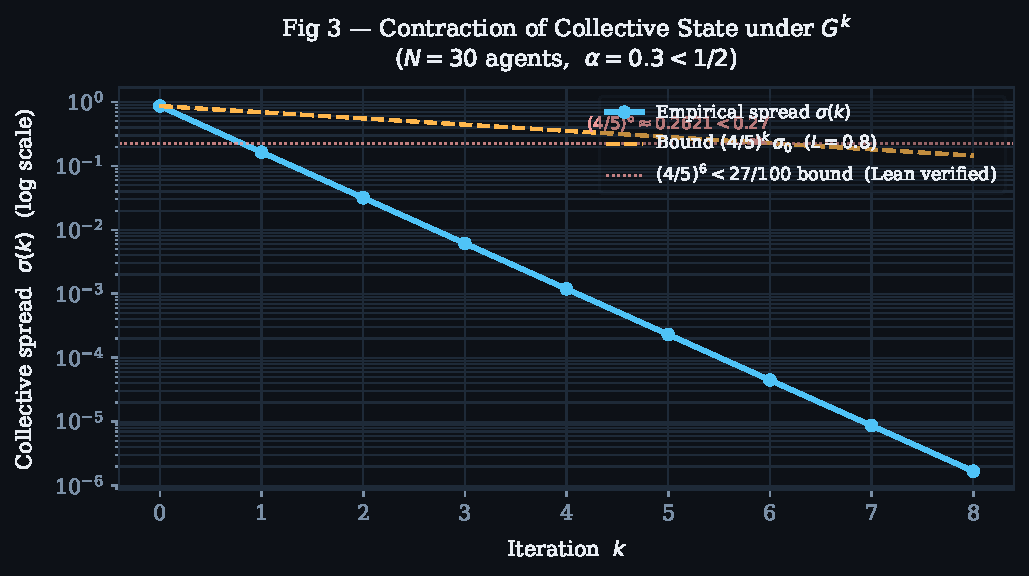
\includegraphics[width=0.92\linewidth]{fig3_convergence.pdf}
  \caption{Contraction of collective spread $\sigma(k)$ under iterated $G$
    (log scale).  The dashed envelope $(4/5)^k\,\sigma_0$ matches the
    theoretical bound; the dotted horizontal marks the
    Lean-verified $(4/5)^6 < 27/100$ bound.}
  \label{fig:conv}
\end{figure}

% ─────────────────────────────────────────────────────────────────────────────
\section{Operator Diagram}
\label{sec:diagram}

Figure~\ref{fig:op} summarises the four-stage pipeline applied to each
biological agent at each generative step.

\begin{figure}[ht]
  \centering
  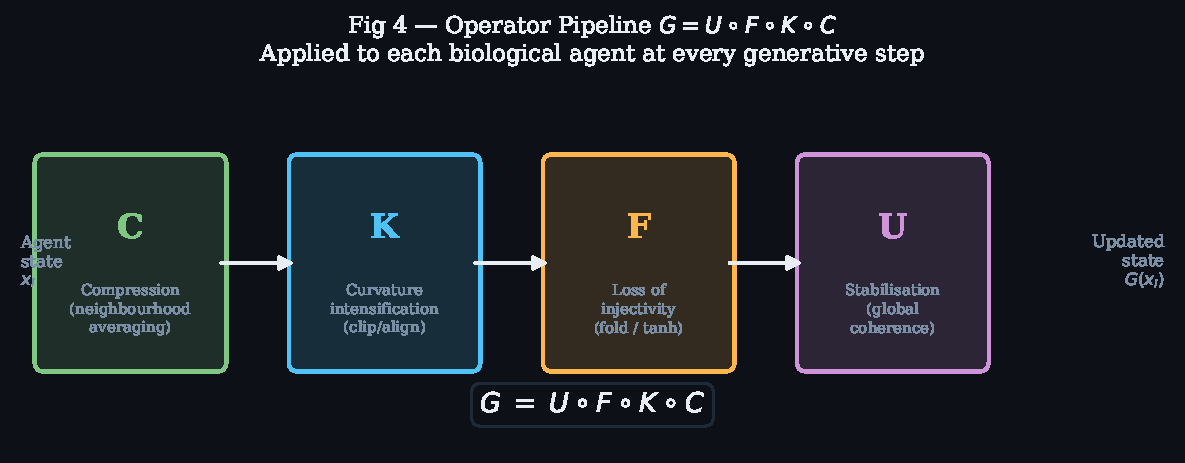
\includegraphics[width=0.97\linewidth]{fig4_operator_diagram.pdf}
  \caption{The operator pipeline $G = U \circ F \circ K \circ C$ applied to a
    single agent state $x_i$ at one generative step.  Left to right: compression
    $C$, curvature intensification $K$, fold $F$, stabilisation $U$.}
  \label{fig:op}
\end{figure}

% ─────────────────────────────────────────────────────────────────────────────
\section{Discussion}
\label{sec:discussion}

The TO/TOGT operator pipeline provides a unified dynamical-systems language for
describing collective biological transitions.  The five case studies
(Sections~\ref{sec:connectome}–\ref{sec:protein}) share the same mathematical
skeleton: agents converge under iterated $G$ to a fixed point or periodic orbit
whose qualitative character (unique, bistable, or oscillatory) is determined
solely by whether $|\alpha|$ falls below, at, or above $\tfrac{1}{2}$.

\paragraph{What the model asserts.}
The model asserts only what Theorem~\ref{thm:contraction} and
Corollaries~\ref{cor:immune}–\ref{thm:six} directly imply: existence and
uniqueness of fixed points, contraction rates, and the pitchfork structure.  No
quantitative biological predictions are made beyond these structural claims.

\paragraph{What the model does not assert.}
The $\dmcube$ numerical invariants $(2\pi, -2, 2)$ are convenience choices, not
predictions.  No claim is made that the Drosophila connectome, the HPA axis, or
the circadian clock are \emph{exactly} described by equation~\eqref{eq:pitchfork}
or Definition~\ref{def:agent}.

\paragraph{Future work.}
Future work will focus on (i) fitting $(\alpha, \varepsilon)$ to empirical
electrophysiology data; (ii) extending the Lean\,4 verification to cover the
biological-scope theorems of this paper; and (iii) experimental falsification of
the predicted bifurcation thresholds.

% ─────────────────────────────────────────────────────────────────────────────
\section*{Acknowledgements}

The author thanks the Zenodo, HAL, and GitHub communities for open-access
infrastructure.  Series root:
\url{https://doi.org/10.5281/zenodo.19117399}.

% ─────────────────────────────────────────────────────────────────────────────
\begin{thebibliography}{99}

\bibitem{vol1}
P.~Nogueira Grossi,
\emph{Principia Orthogona, Volume One: The Mathematics of Generative
Transitions},
HAL hal-05555216v1, March 2026.

\bibitem{vol2}
P.~Nogueira Grossi,
\emph{Principia Orthogona, Volume Two: Contact Realisation of Generative
Transitions},
HAL hal-05559997v1 / hal-05565024v1, March 2026.

\bibitem{companion}
P.~Nogueira Grossi,
\emph{Biological Transitions: Fruit-Fly Connectome Toy Model (Drosophila) ---
V2 Complete},
Zenodo \href{https://doi.org/10.5281/zenodo.19210136}{10.5281/zenodo.19210136},
2026.

\bibitem{flywire2023}
D.~Dorkenwald \emph{et al.},
\emph{Neuronal wiring diagram of an adult brain},
Nature \textbf{625}, 654--664 (2024).
\href{https://doi.org/10.1038/s41586-023-06979-1}{doi:10.1038/s41586-023-06979-1}

\bibitem{sapolsky2004}
R.~M.~Sapolsky,
\emph{Why Zebras Don't Get Ulcers},
3rd ed., W.\,H.~Freeman, 2004.

\bibitem{pittendrigh1960}
C.~S.~Pittendrigh,
Circadian rhythms and the circadian organization of living systems,
\emph{Cold Spring Harbor Symp.\ Quant.\ Biol.}\ \textbf{25}, 159--184 (1960).

\bibitem{burnet1959}
F.~M.~Burnet,
\emph{The Clonal Selection Theory of Acquired Immunity},
Cambridge University Press, 1959.

\bibitem{anfinsen1973}
C.~B.~Anfinsen,
Principles that govern the folding of protein chains,
\emph{Science} \textbf{181}(4096), 223--230 (1973).

\end{thebibliography}

\end{document}
